\documentclass[11pt,titlepage,a4paper]{article}

\usepackage[utf8]{inputenc}
\usepackage{mathtools}
\usepackage{amsmath}
\usepackage{amssymb}
\usepackage{xcolor}
\usepackage{multirow}
\usepackage{float}
\usepackage{array}
\usepackage{graphicx}
\usepackage{epstopdf}
\usepackage{graphics}
\usepackage{tabu}
\usepackage{titlesec}
\usepackage[titletoc,toc,title]{appendix}
\usepackage[textwidth=6.4in]{geometry}
\usepackage{color}
\usepackage{hyperref}
\usepackage{cleveref}
%\usepackage{autonum}
\usepackage{tabularx}
\usepackage{caption}
\usepackage{subcaption}
%\usepackage[format=plain, font=it]{caption}
\usepackage{wasysym}
\usepackage{csvsimple}
\usepackage{longtable}
\usepackage{titling}
\usepackage{caption}
\usepackage{subcaption}
\usepackage[
    backend=biber,
    style=apa
    ]{biblatex}
\addbibresource{Sections/References.bib}

\usepackage{listings}
\usepackage{xcolor}

\definecolor{codegreen}{rgb}{0,0.6,0}
\definecolor{codegray}{rgb}{0.5,0.5,0.5}
\definecolor{codepurple}{rgb}{0.58,0,0.82}
\definecolor{backcolour}{rgb}{0.95,0.95,0.92}

\lstdefinestyle{mystyle}{
    backgroundcolor=\color{backcolour},   
    commentstyle=\color{codegreen},
    keywordstyle=\color{magenta},
    numberstyle=\tiny\color{codegray},
    stringstyle=\color{codepurple},
    basicstyle=\footnotesize,
    breakatwhitespace=false,         
    breaklines=true,                 
    captionpos=b,                    
    keepspaces=true,                 
    numbers=left,                    
    numbersep=5pt,                  
    showspaces=false,                
    showstringspaces=false,
    showtabs=false,                  
    tabsize=2
}
 
\lstset{style=mystyle}

\newcommand{\inputCodeFile}[1]{
    \lstinputlisting[numbers=left,breaklines,breakatwhitespace,language=Python]{#1}
}

%-------------------------------------------------------------------------------------------------------

\renewcommand{\contentsname}{Table of contents}

\def\mapmatter{%
    \pagenumbering{gobble}
}%

\def\mainmatter{%
    \pagenumbering{arabic}
    \setcounter{page}{1}
    \setcounter{section}{0}
    \renewcommand{\thesection}{\arabic{section}}
}%

\def\backmatter{%
    \setcounter{section}{0}
    \renewcommand{\thesection}{\Alph{section}}
}%



%-------------------------------------------------------------------------------------------------------


% counters
\newcounter{exercise}
\newcounter{subexercise}

\newcommand{\newSub}{
    \refstepcounter{subexercise}\par\medskip
    \noindent
    \textbf{\theexercise.\alph{subexercise})}
}

% Environments
\newenvironment{exercise}{
    \refstepcounter{exercise}\par\medskip
    \noindent
    \textbf{Exercise~\theexercise}
    \newline
    \noindent
}{
    \medskip
    \setcounter{subexercise}{0}
}

\newcommand{\Null}[1]{\text{Null}\left(#1\right)}
\newcommand{\Col}[1]{\text{Col}\left(#1\right)}
\newcommand{\argmin}[1]{\underset{#1}{\text{argmin}}}
\newcommand{\Cov}[1]{\text{Cov}\left[#1\right]}
\newcommand{\lone}{\ell_1}
\newcommand{\betah}{\hat{\beta}}
\newcommand{\sign}[1]{\text{sign}\left(#1\right)}


\newcommand{\maxDepth}{\textit{max\_depth} }
\newcommand{\nEstimators}{\textit{n\_estimators} }
\newcommand{\maxSamples}{\textit{max\_samples} }

\begin{document}
    % TitlePage
    \begin{titlepage}
    \vspace{\fill}
    \centering
    
    % Rule
    \par\noindent\rule{\textwidth}{0.4pt}
    \par\noindent\rule{\textwidth}{0.4pt}

    \vspace{0.5cm}
    
    % Title
    {
        \Huge 
        Prediction and modelling of mortgage prepayment risk
    }

    \vspace{0.5cm}

    % Rule
    \par\noindent\rule{\textwidth}{0.4pt}
    \par\noindent\rule{\textwidth}{0.4pt}
    
    \vspace{3cm}

    % Names
    {
        \large 
        Aristos Kaloudis 5364493 \\
        Tom Heijnders 4362659 \\
        Sebastiaan van Schagen 4684877 \\
        Raoul Roest 4299086
    }

    \vspace{1cm}

    % Supervisor
    {
        \large Supervisor:\\ 
        Dr. D. Kurowicka (TUDelft)
    }
    
    \vspace{1cm}

    % Date
    \today

    \vspace{3cm}
    
    % Images
    \begin{figure}[H]    
        \centering
        % Delft image
        \begin{minipage}{0.4\textwidth}
            
\includegraphics[width=6cm]{Figures/TU_Delft_logo_RGB.png}
        \end{minipage}
        \hfill
        % Deloitte image
        \begin{minipage}{0.4\textwidth}
            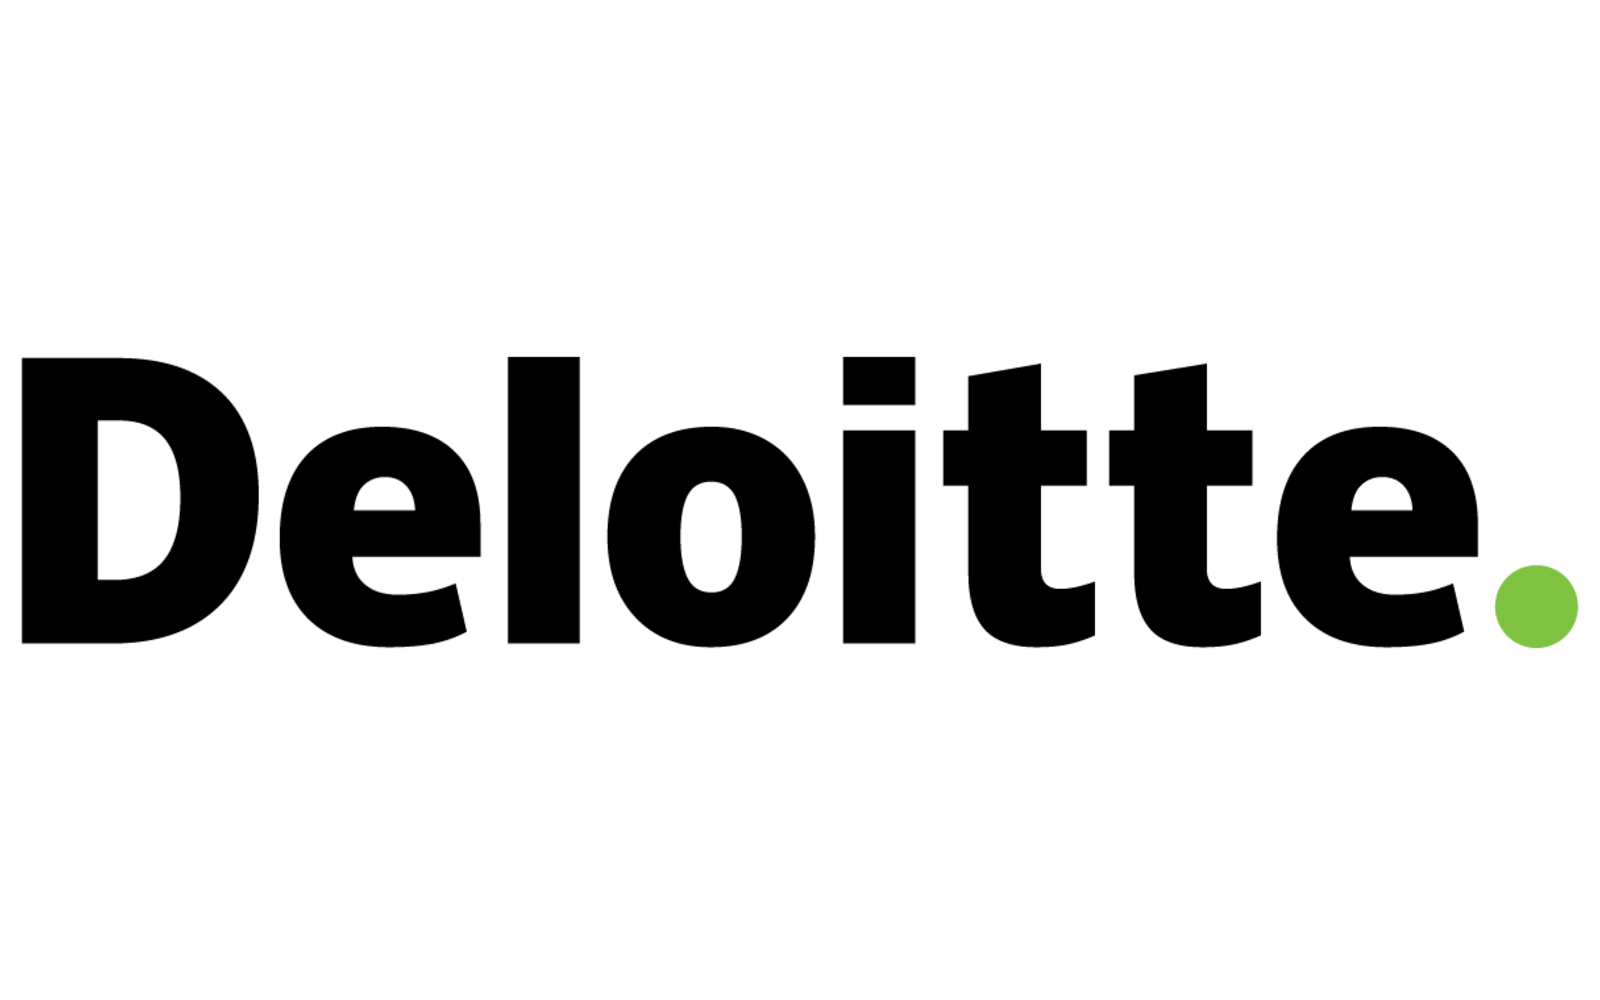
\includegraphics[width=5cm]{Figures/Logo_Deloitte.png}
        \end{minipage}
    \end{figure}

    \vfill

\end{titlepage}


    % TOC
    \tableofcontents

    \newpage
    
    % Sections
    \section{Introduction}\label{section_introduction}
    A mortgage loan is a common agreement between two parties: the lender and the borrower. 
The lender, mostly banks, lends money to the borrower. The money is 
secured with collateral and in case of default or regular failure to follow 
the agreed payment schedule, the collateral could be sold to obtain the outstanding amount. Within the mortgage 
agreement, a series contractual payments is used to repay the mortgage. 
The contractual payments consist of repayment of the 
mortgage and interest calculated over the outstanding debt. 
The interest can be divided into two groups, one considers a 
fixed interest rate and the other a non-fixed interest rate. The 
interest rate determines the profit of het lender. 
\\\\
A lender takes several risks such as a failing payment of the loanee or 
changing interest rates. Another risk is the loanee to prepay. Repaying 
is paying a part of the borrowed money before the agreed date of the 
scheduled payments. One speaks of partial prepayment when a part of 
the outstanding debt is prepaid. Likewise, a full prepayment is defined 
as prepaying the remaining debt. There is a possibility for the lender 
to charge extra costs for the prepayments. Both the interest and the 
scheduled payments form the income on the lender. If the loanee decides 
to prepay, the interest rate obtained becomes smaller and income 
decreases.  On small scales this gives no problems, however, instead 
of one loanee, a bank can write mortgages to many loanees at once. 
This can result in big losses in comparison to the expected income.  
\\\\
As behaviour of clients can be predicted, extra funds could be kept 
separate to decrease risk without keeping unnecessary reserves. In this 
report there is looked at open-source data collected by FreddieMac and 
aimed to predict prepayments based on this data. The prediction is 
based on lender level. We want to predict prepayments in the next 
timestep for a given time. First, the data is analysed in Section 
\ref{section_data_analysis}. In which also the prepayment rule is 
derived. Followed by the model and performance criteria in Section 
\ref{section_model}. Next, the obtained results are shown in 
Section \ref{section_results}. Last, a discussion is formed, 
consisting of a conclusion, improvements and extensions of the model 
in Section \ref{section_discussion}.
\\\\
Special thanks to:\\
Dr. D. Kurowicka (TUDelft)\\
R. Tuinhof (Deloitte)\\
R. van der Leij (Deloitte)

    \newpage
    
    \section{Data analysis}\label{section_data_analysis}
    In this section, preparation work is completed. First, the data is cleaned and analysed. Followed by observation in the data. Next, the derivation of the prepayments is shown.  

\subsection{Data description}
    The data collected by FreddieMac consist of two files, a loan originated file and a monthly payment file. FreddieMac continuously updates and corrects the files to keep them up to date. In this report, sample data of years 2013-2020 is used in which each year corresponds to 50000 loans (with an exception for 2020). The origination file corresponds to the origin of the loan and thus loanee. This data does not change over time. The origination file consists of 31 characteristics of a loan: credit score (FICO), first payment date, first time homebuyer flag, maturity date, Metropolitan statistical area (MSA), mortgage insurance percentage, number of units, occupancy status, original combined loan-to-value (CLTV), original debt-to-income rate (DTI), original UPB, original loan-to-value (LTV), original interest rate, channel, prepayment penalty mortgage flag (PPM), amortization type, property state, property type, postal code, loan sequence number, loan purpose, original loan term, number of loanees, seller name, servicer name, super conforming flag, pre-HARP loan sequence number, program indicator HARP indicator, property valuation method and interest only indicator. For an explanation of the characteristics see user guide provided by FreddieMac. Not all these characteristics are relevant to predict future prepayment and some are removed out of the data. Pre-HARP, HARP indicator and interest only indicator are removed.
    \\\\
    Additional to the origination file, the monthly performance file is given. The monthly performance file consist of the data dependent on time. The data of every loan is monthly determined from the first payment data until 2020. If the mortgage is fully repaid due to full prepayment or the maturity date is reached, the monthly performance of that loan is stopped. The monthly performance file consist of 30 characteristics: Loan sequence number, monthly reporting period, current actual UPB, current loan delinquency status, loan age, remaining months to legal maturity, repurchase flag, modification flag, zero balance code, zero balance effective date, current interest rate, current deferred UPB, due date of last pain instalment (DDLPI), MI recoveries, net sale  proceeds, non MI recoveries, expenses, legal costs, maintenance and preservation costs, taxes and insurance, miscellaneous expenses, actual loss calculation, modification cost, step modification flag, deferred payment plan, estimated loan to value (ELTV), zero balance removal UPB, delinquent accrued interest, delinquency due to disaster, loanee assistance status code. For an explanation of the characteristics see user guide provided by FreddieMac. Again, some characteristics are removed out of the data. In the monthly performance file, MI recoveries, net sale proceeds, non-MI recoveries, expenses, legal costs, maintenance and preservation costs, taxes and insurance, miscellaneous expenses, actual loss calculation and delinquent accrued interest are removed. 

\subsection{Data cleaning}
	Some irrelevant data is already removed out of the data, however, there is still some cleaning to do. In both files some characteristics of the loan are standardized if not available. These loans cannot be used to predict future prepayments and need to be removed out of the data. The loans corresponding to undefined data of characteristics FICO, CLTV, DTI, LTV, property type and PPM are removed out of the data. Besides, there is only interest for prepayment or matured mortgages, hence we filter on the zero-balance code. The zero-balance code is a code implying what happened to the mortgage. We obtain of 373602 loans fitted to predict prepayments, see Table \ref{model_cleaned data_table} for the distribution over the years. 
    \begin{table}[H]
        \centering
        \begin{tabular}{c|c}
            Year & Number of loans \\\hline
            2013 & 49835 \\
            2014 & 49821 \\
            2015 & 49871 \\
            2016 & 49878 \\
            2017 & 49836 \\
            2018 & 49841 \\
            2019 & 49698 \\
            2020 & 24822 \\\hline
            Total & 373602 
		\end{tabular}
		\caption{Number of loans for years 2013-2020 after cleaning the data.}
		\label{model_cleaned data_table}
    \end{table}
    
\subsection{Prepayment derivation}
    As mentioned, prepayment is defined as paying a part of a loan in advance. Before something can be seen as a prepayment, the original payment needs to be determined.
    The annuity mortgage is characterize by its equal payments. 
Suppose payments $B_1, \ldots, B_n$, for these payments the relation
\begin{equation}
    B_1 = \ldots = B_n 
\end{equation}
holds. Note that at $t_0$ there is no payments (as the mortgage is granted).
Let us denote the interest at time $t$ as $r_t$. Since we look at fixed mortgages 
the relation
\begin{equation}
    r_1 = \ldots = r_n
\end{equation}
holds for the interest rates. 
Let us assume that we are in a risk neutral market. When we valuate the loan in the risk 
neutral market, the present value of the outstanding debt, should be equal to the loan
and hence
\begin{equation}
    L = B (1 + r)^{-t_1} + \ldots B (1 + r)^{-t_n}
\end{equation}
where $L$ is the granted loan. Using the geometric series, the value of each payment 
$B$ can be determined: 
\begin{equation}
    B\left[
        \displaystyle\sum_{j=1}^{n} (1 + r)^{-t_j}  
    \right] = 
    B\left[
        \displaystyle\sum_{j=0}^{n} (1 + r)^{-t_j} - 1  
    \right] = 
    B \left[
        \dfrac{1 - (1 + r)^{n+1}}{1 - (1 + r)} - 1
    \right] =
    B \left[
        \dfrac{1 - (1 + r)^{n+1}}{r}  - 1
    \right].
\end{equation}
From this the monthly payments $B$ can be determined: 
\begin{equation}
    B = \dfrac{L}{
        \left(
            \dfrac{1 - (1 + r)^{n+1}}{r} - 1
        \right)
    }
\end{equation}
The term 
\begin{equation}
    \dfrac{1 - (1 + r)^{n+1}}{r} - 1        
\end{equation}
will we call the monthly factor. Note that the interest rate given is a yearly rate. The 
corresponding monthly rate can be calculated by: 
\begin{equation}
    (1 + r)^{\frac{1}{12}}.
\end{equation} 
    \\\\
    Now we know how to see prepayments, however this needs to be applied to the monthly performance data. The amount paid at a month is calculated for every month. If the amount paid is bigger than a threshold times the predefined monthly payment, the maturity data is not reached and if the number of days the loanee is delinquent is less than 30 days, then it is considered as a prepayment. The threshold ensures some freedom in the series of payments. For example, if the loanee does not pay in one month and pays double in the following month, it should not be considered as a prepayment. If the remaining debt after the prepayment becomes zero, it is considered as a full prepayment. Every other prepayment is denoted as partial prepayment. In Table \ref{model_classficationprepayment_table}, the number of loans with prepayments can be found. Loan consisting of no prepayments or full prepayments are appearing most in the sample data. 
    \begin{table}[H]
    \centering
    \begin{tabular}{c|c|c|c|c}
        & \multicolumn{4}{c}{Number of loans} \\
        Year&No Prepayment&Partial Prepayment&Full Prepayment&Partial \& Full prepayment  \\\hline
        2013 & 20783 & 4159 & 22136 & 2757\\
        2014 & 17909 & 3082 & 26537 & 2293\\
        2015 & 24027 & 3365 & 20811 & 1668 \\
        2016 & 28984 & 3137 & 16603 & 1154 \\
        2017 & 29460 & 2479 & 16959 & 938 \\
        2018 & 27368 & 1764 & 19901 & 808 \\
        2019 & 37041 & 1049 & 11426 & 182 \\
        2020 & 24160 & 39 & 623 & 0 \\
        Total & 209732 & 19074 & 134996 & 9800
		\end{tabular}
		\caption{Classification of loans for years 2013-2020 with threshold percentage of 0.1.}
		\label{model_classficationprepayment_table}
    \end{table}

\subsection{Time dependence of the data}
    As can seen in Table \ref{model_cleaned data_table}, sample data of every year consist of roughly 50000 loans. The exception is 2020 as this is involves recent loans and first the data needs to be gathered. For every year we observe a similar distribution of prepayments. However, there is some nuance. As time goes by, more loanees starts to prepay. Loanees getting a mortgage in 2013 are more likely to have prepaid an amount than loanees with a mortgage originating of 2020. This does however not change the potential risk drivers. During these years, nothing special happened which had a large impact on the economic system. Note, we are working with a small part of 2020. In general, we can assume the behaviour to be similar through the years.
    \textcolor{red}{Picture obtained by Tom!}

\subsection{Importances of the data}
    To ensure privacy, some characteristics of a loan and loanee are made general and hence difficult to work with. Some drivers of prepayment could be age and income of the loanee. Someone with a higher income is more likely to prepay, similar, someone older is more likely to have some extra money and thus possible prepay. However, these characteristics are not directly available in the data. Income is used to calculate several measures, but not given specifically. Age is never mentioned in the data although it is useful to predict prepayments.  

    Although there is some relevant data missing, this data format is used in the remainder of the report.  However, there is something wrong with the starting lines of the monthly performance files. In some cases, the current UPB rounded to the nearest thousand. This results in some strange behaviour of the payments of the loanees and need to be dealt with. There need to be set a bound to the classification of prepayments. This can be solved with use of a threshold as discussed later. 
    \\\\
    We discuss a small selection of characteristics of a loan, other characteristics behave similar and seem independent of prepayments. For a complete variable importance determination, see Section \ref{section_model}. 
    
    \subsubsection{Original loan-to-value}
        Some characteristics of a loan are obtained with similar data and thus might be dependent. For example, both LTV and CLTV are calculated using similar characteristics: 
        \\\\
        Some characteristics of a loan are obtained with similar data and thus might be dependent. For example, both LTV and CLTV are calculated using similar characteristics: 
        \begin{align}
            \text{LTV}&=\frac{\text{Original loan amount}}{\text{Purchase price}}\\
            \text{CLTV}&=\frac{\text{Original loan amount}+\text{Secondary loan amount}}{\text{Purchase price}}\\
            &\text{If } LTV \leq CLTV, CLTV \text{ is denoted as unavailable}
        \end{align}
    
    
        To discover the behaviour of LTV in case of partial and full prepayments, a boxplot is made. In Figure \ref{model_boxplot_LTV} the boxplot shows that there is significant difference in the behaviour of the LTV in cases of no prepayment compared to partial and full prepayments. Besides, performing a Kolmogorov Smirnov test and obtain the p-values as given in Table \ref{model_Pvals_of_LTV}. All p-values are zero implying independent data. A zero p-value could however, also correspond to too much data. 
        \begin{table}[H]
        \centering
            \begin{tabular}{lcl|c|c}
            \multicolumn{3}{c}{Prepayment type} & P-values& KS-statistic \\\hline
            No Prepayment & \& & Full Prepayment & 0 & 0.064475\\
            No Prepayment & \& & Partial Prepayment & 0 & 0.091396\\
            No Prepayment & \& & Full or Partial Prepayment & 0 & 0.048204 \\
            Full Prepayment & \& & Partial Prepayment & 0 & 0.146167
		    \end{tabular}
            \caption{P-values of LTV (in which if both partial and full prepayments happen, it is denoted as full prepayment).}
	        \label{model_Pvals_of_LTV}
        \end{table}
    
        \begin{figure}[H]
            \centering
            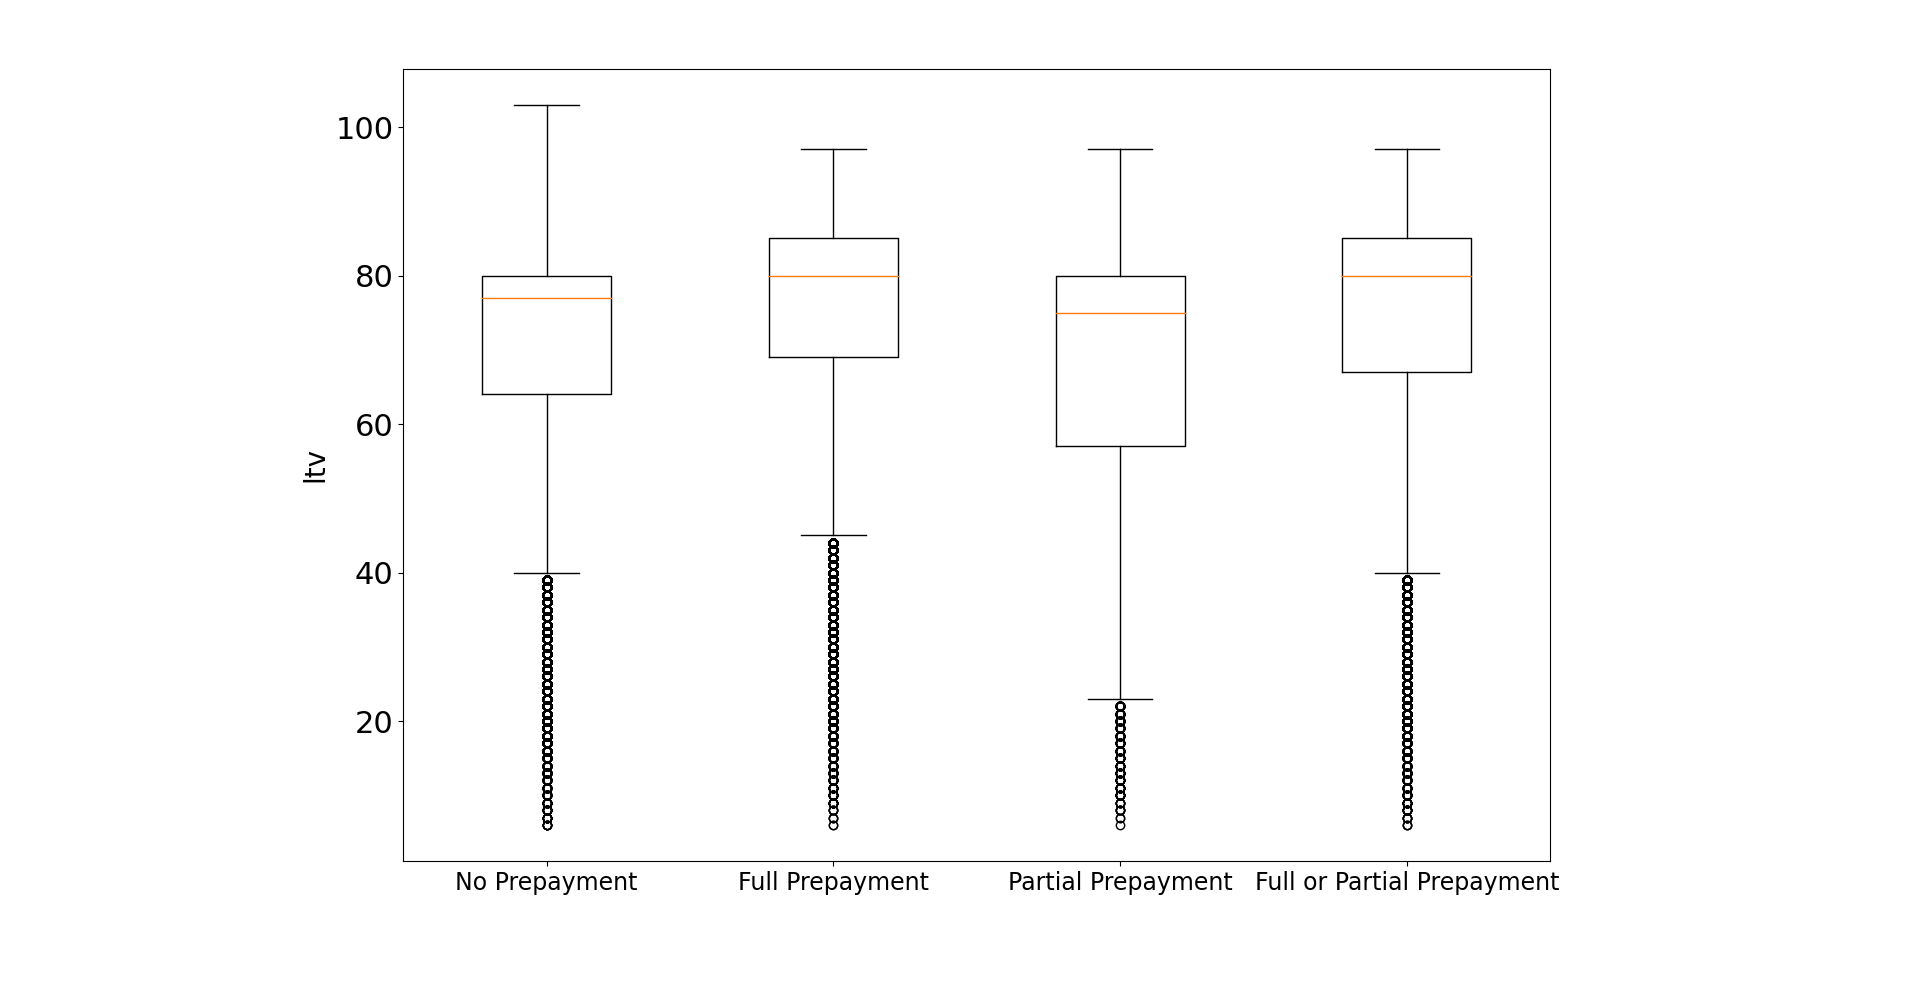
\includegraphics[width=\linewidth]{Latex/Report/Figures/Boxplot_of_ltv_[2013, 2014, 2015, 2016, 2017, 2018, 2019, 2020]_.png}
            \caption{Boxplot of LTV for sample data. From left to right: No prepayment, Full prepayment, Partial prepayment and Full or Partial prepayment.}
            \label{model_boxplot_LTV}
        \end{figure}
    
        \noindent
        Combining Figure \ref{model_boxplot_LTV} and Table \ref{model_Pvals_of_LTV}, LTV can be considered as a potential risk driver and needs further investigation. As mentioned, one observes similar behaviour of the data through the years. For further investigation, we consider year 2013 as all other years give similar results.  
    
        In Figure \ref{model_LTV_against_prepayment} the loans in which no prepayments are made are filtered out of the data. We observe higher magnitudes for LTV values around 80, which is in accordance with Figure \ref{model_boxplot_LTV}. This figures implies again that LTV could be a risk driver. 
        \begin{figure}[H]
            \centering
            \begin{subfigure}{0.45\textwidth}
                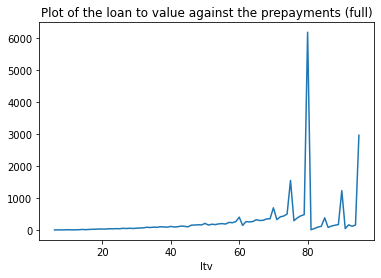
\includegraphics[width=\linewidth]{Latex/Report/Figures/LTV againts Full prepayments.png}
                \caption{LTV against Full prepayments.}
                \label{model_LTV_against_full_prepayment}
            \end{subfigure}
            \begin{subfigure}{0.45\textwidth}
                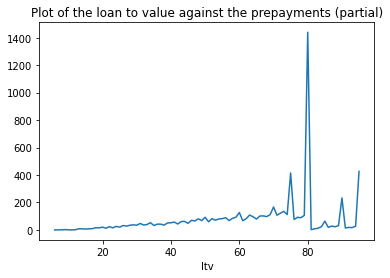
\includegraphics[width=\linewidth]{Latex/Report/Figures/LTV againts Partial prepayments.png}
                \caption{LTV against Partial prepayments.}
                \label{model_LTV_against_partial_prepayment}
            \end{subfigure}
            \caption{LTV against magnitude of prepayments.}
            \label{model_LTV_against_prepayment}
        \end{figure}
    
    \subsubsection{Original combined loan-to-value}
        As stated, both CLTV and LTV are calculated in similar ways. To study the behaviour of CLTV in case of partial and full prepayments, a boxplot is made. In Figure \ref{model_boxplot_CLTV} one obverses a difference in behaviour. This behaviour is tested using Kolmogorov Smirnov test as well, the obtained p-values can be found in Table \ref{model_Pvals_of_CLTV}. All p-values are zero which suggest independent data. A zero p-value could however, correspond to too much data, as well.
        \begin{table}[H]
        \centering
            \begin{tabular}{lcl|c|c}
            \multicolumn{3}{c}{Prepayment type} & P-values& KS-statistic \\\hline
            No Prepayment & \& & Full Prepayment & 0 & 0.070947\\
            No Prepayment & \& & Partial Prepayment & 0 & 0.090918\\
            No Prepayment & \& & Full or Partial Prepayment & 0 & 0.053969 \\
            Full Prepayment & \& & Partial Prepayment & 0 & 0.150986
		    \end{tabular}
            \caption{P-values of CLTV (in which if both partial and full prepayments happen, it is denoted as full prepayment).}
	        \label{model_Pvals_of_CLTV}
        \end{table}
        Further investigating year 2013 we observe similar behaviour for CLTV, see Figure \ref{model_CLTV_against_prepayment}. This behavior is similar as with LTV.
        \begin{figure}[H]
            \centering
            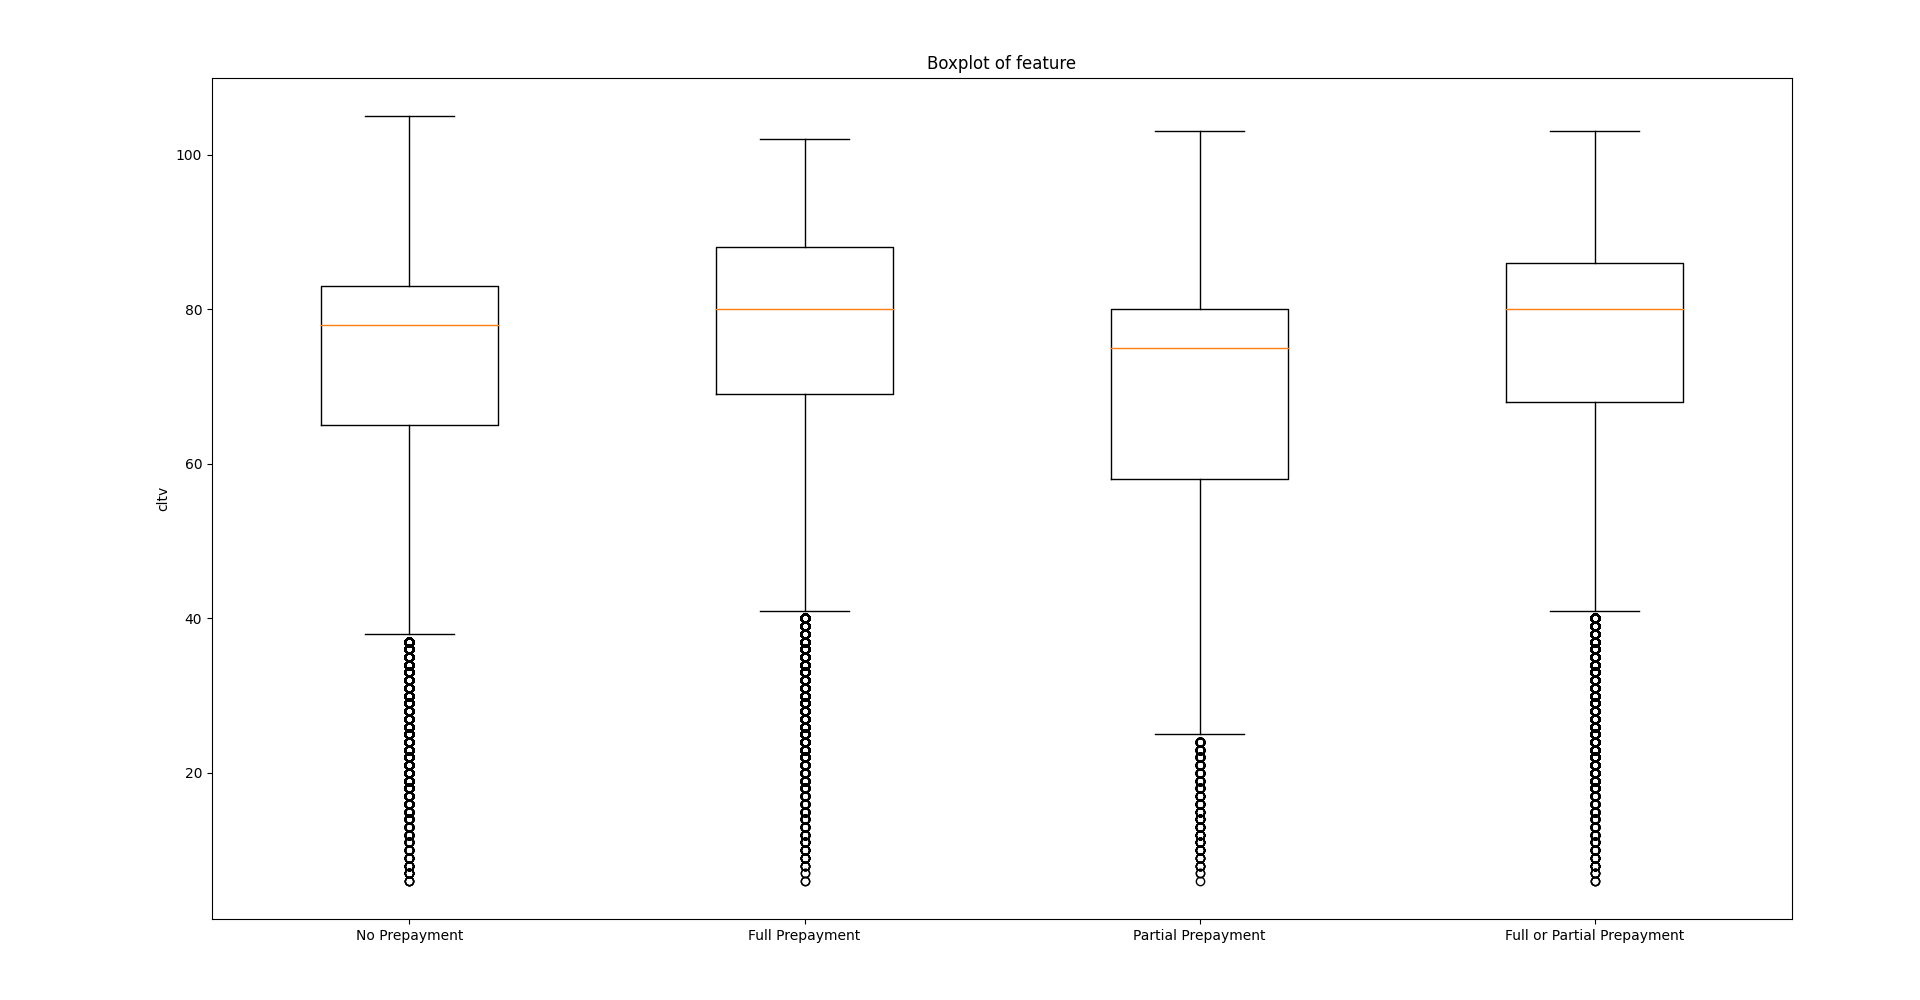
\includegraphics[width=\linewidth]{Latex/Report/Figures/Boxplot_of_cltv_[2013, 2014, 2015, 2016, 2017, 2018, 2019, 2020]_.png}
            \caption{Boxplot of CLTV of sample data. From left to right: No prepayment, Full prepayment, Partial prepayment and Full or Partial prepayment.}
            \label{model_boxplot_CLTV}
        \end{figure}
        \begin{figure}[H]
            \centering
            \begin{subfigure}{0.45\textwidth}
                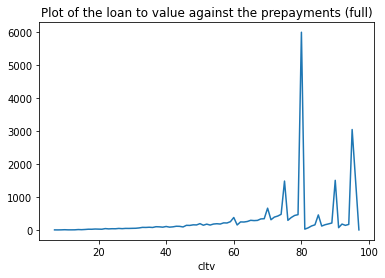
\includegraphics[width=\linewidth]{Latex/Report/Figures/CLTV againts Full prepayments.png}
                \caption{CLTV against Full prepayments.}
                \label{model_CLTV_against_full_prepayment}
            \end{subfigure}
            \begin{subfigure}{0.45\textwidth}
                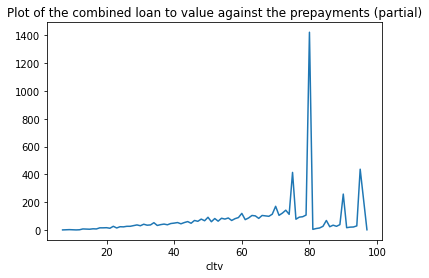
\includegraphics[width=\linewidth]{Latex/Report/Figures/CLTV againts Partial prepayments.png}
                \caption{CLTV against Partial prepayments.}
                \label{model_CLTV_against_partial_prepayment}
            \end{subfigure}
            \caption{CLTV against magnitude of prepayments.}
            \label{model_CLTV_against_prepayment}
        \end{figure}
        
    \subsubsection{Original unpaid principal balance}
        Another important characteristic of a loan is the UPB, which denotes the value of the mortgage. This characteristic is used to calculate both LTV and CLTV. From the observations of CLTV and LTV it is expected that a loan with high UPB with small purchase price is more likely to be prepaid. However, a low UPB is also likely to be prepaid as the money required to make a prepayment is less in comparison to a high UPB. To see if this is in accordance with the data a boxplot consisting all sorts of prepayments is formed. In Figure \ref{model_boxplot_UPB} one sees the UPB corresponding to partial prepayments to be smaller than the UPB of no prepayments. Which is in accordance with our last remark about the behaviour of the UPB. On the other hand, the UPB corresponding to full prepayments turns out to be higher than the UPB of no prepayments. This is already observed in the behaviour of LTV and CLTV. 
        \begin{figure}[H]
            \centering
            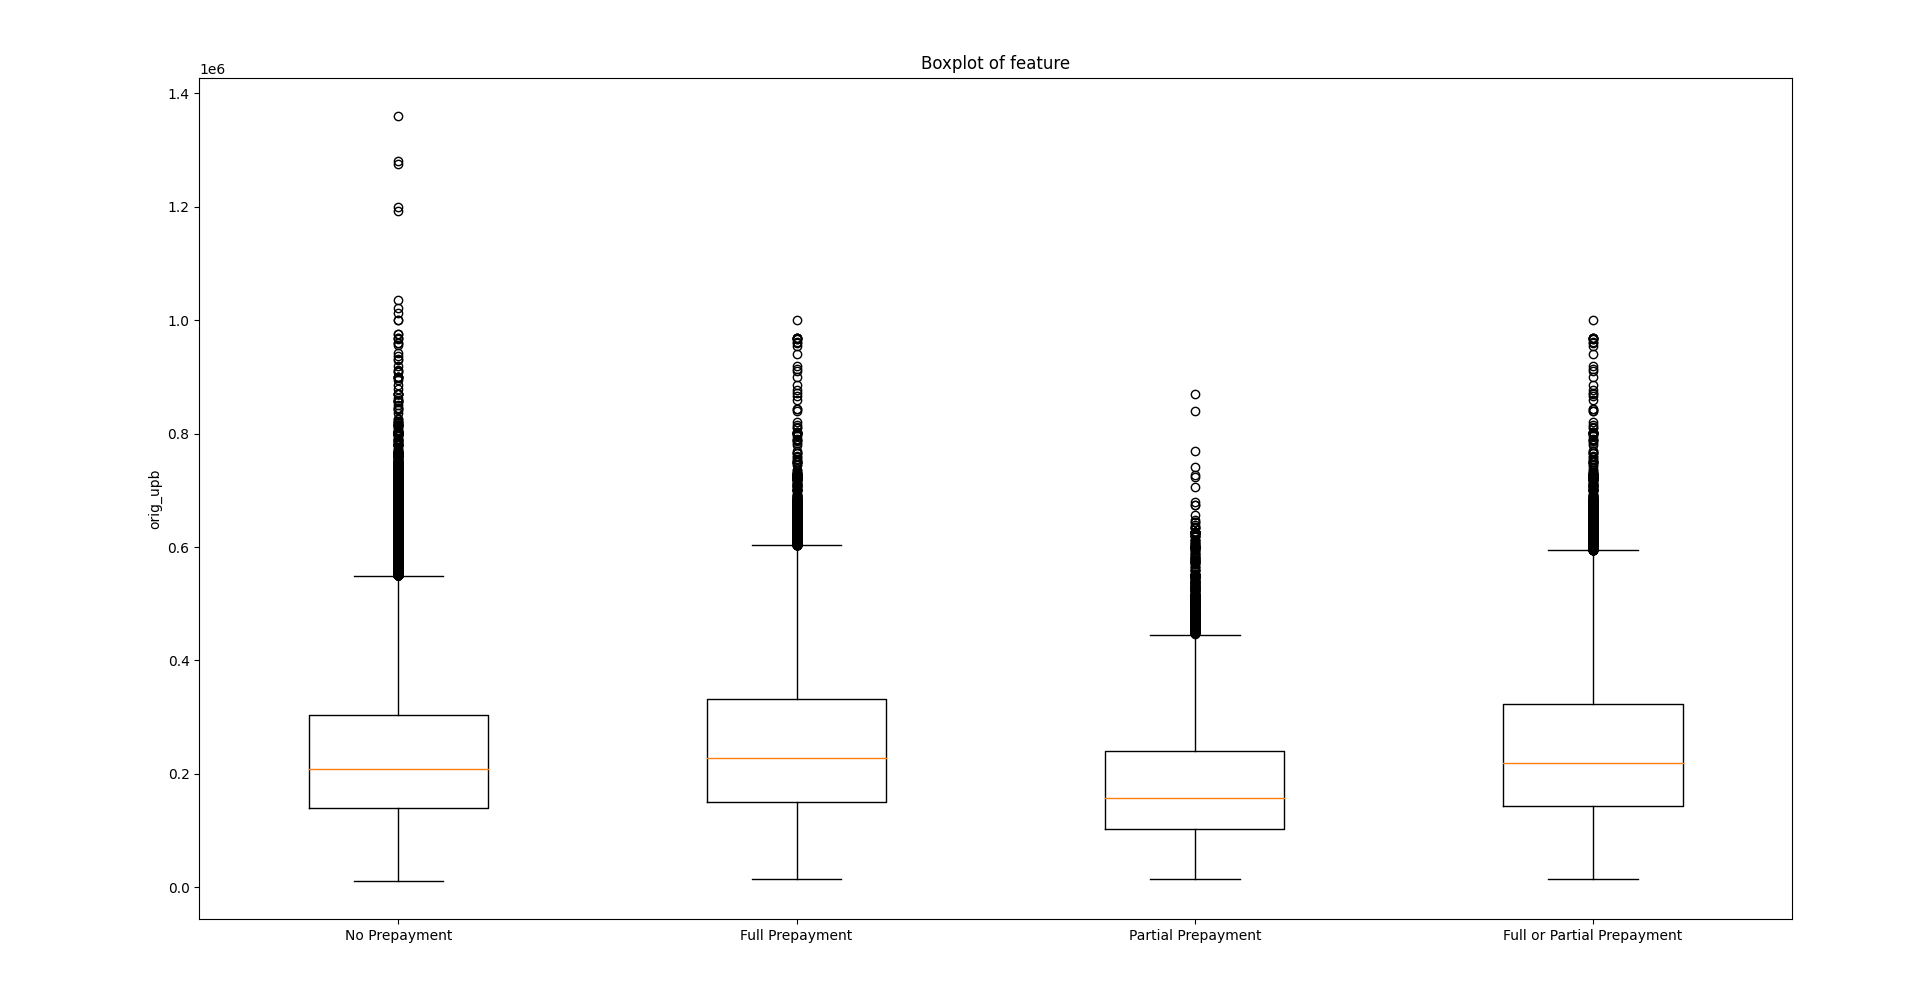
\includegraphics[width=\linewidth]{Latex/Report/Figures/Boxplot_of_upb_[2013, 2014, 2015, 2016, 2017, 2018, 2019, 2020]_.png}
            \caption{Boxplot of UPB for sample data. From left to right: No prepayment, Full prepayment,Partial prepayment and Full or Partial prepayment.}
            \label{model_boxplot_UPB}
        \end{figure}
        \noindent
        The dependence of the UPB is determind with use of Kolmogorov Smirnov test, as well. In Table \ref{model_Pvals_of_UPB}, all p-values are zero and hence the data is independent. A zero p-value could however, also correspond to too much data. 
        \begin{table}[H]
        \centering
            \begin{tabular}{lcl|c|c}
            \multicolumn{3}{c}{Prepayment type} & P-values& KS-statistic \\\hline
            No Prepayment & \& & Full Prepayment & 0 & 0.068385\\
            No Prepayment & \& & Partial Prepayment & 0 & 0.182088\\
            No Prepayment & \& & Full or Partial Prepayment & 0 & 0.043719 \\
            Full Prepayment & \& & Partial Prepayment & 0 & 0.238933
		    \end{tabular}
            \caption{P-values of UPB (in which if both partial and full prepayments happen, it is denoted as full prepayment).}
	        \label{model_Pvals_of_UPB}
        \end{table}
        \noindent
        By isolation the data of year 2013, we observe the result given in Figure         \ref{model_UPB_against_prepayment}. Here we clearly see a smaller UPB resulting in more prepayments. We can conclude that UPB is an important characteristic to predict prepayments. 
        \begin{figure}[H]
            \centering
            \begin{subfigure}{0.45\textwidth}
                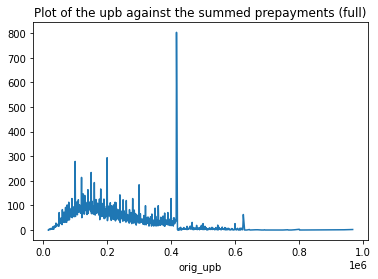
\includegraphics[width=\linewidth]{Latex/Report/Figures/UPB againts Full prepayments.png}
                \caption{UPB against Full prepayments.}
                \label{model_UPB_against_full_prepayment}
            \end{subfigure}
            \begin{subfigure}{0.45\textwidth}
                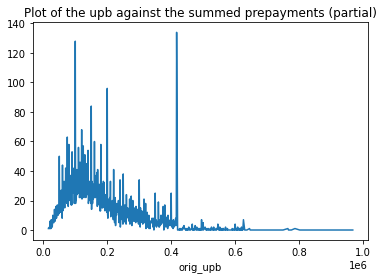
\includegraphics[width=\linewidth]{Latex/Report/Figures/UPB againts Partial prepayments.png}
                \caption{UPB against Partial prepayments.}
                \label{model_UPB_against_partial_prepayment}
            \end{subfigure}
            \caption{UPB against magnitude of prepayments.}
            \label{model_UPB_against_prepayment}
        \end{figure}
        
    \subsubsection{Original interest rate}
    At last, we consider the behaviour of characteristic original interest rate. It is expected that in loans with a higher interest rate, more prepayments are made. This follows from getting a loan somewhere else with lower interest rate and using this money to prepay the original loan. The data is split based on the kind of prepayment. This division is used to determine possible dependence between this characteristic. The p-values given in Table \ref{model_Pvals_of_int} suggest the data to be independent. This test is performed on a large amount of data and hence might be false. 
    \begin{table}[H]
        \centering
            \begin{tabular}{lcl|c|c}
            \multicolumn{3}{c}{Prepayment type} & P-values& KS-statistic \\\hline
            No Prepayment & \& & Full Prepayment & 0 & 0.195919\\
            No Prepayment & \& & Partial Prepayment & 0 & 0.079967\\
            No Prepayment & \& & Full or Partial Prepayment & 0 & 0.165275 \\
            Full Prepayment & \& & Partial Prepayment & 0 & 0.263374
		    \end{tabular}
            \caption{P-values of interest rates (in which if both partial and full prepayments happen, it is denoted as full prepayment).}
	        \label{model_Pvals_of_int}
        \end{table}
        \noindent
        A boxplot comparing the prepayment might back up the p-values. In Figure \ref{model_boxplot_int_rt}, a difference of behaviour is seen based on the type of prepayment. A prepayment happens more likely when the original interest rate is high. Which is as expected. However, the partial prepayments turn out to be made with smaller original interest rates. 
        \begin{figure}[H]
            \centering
            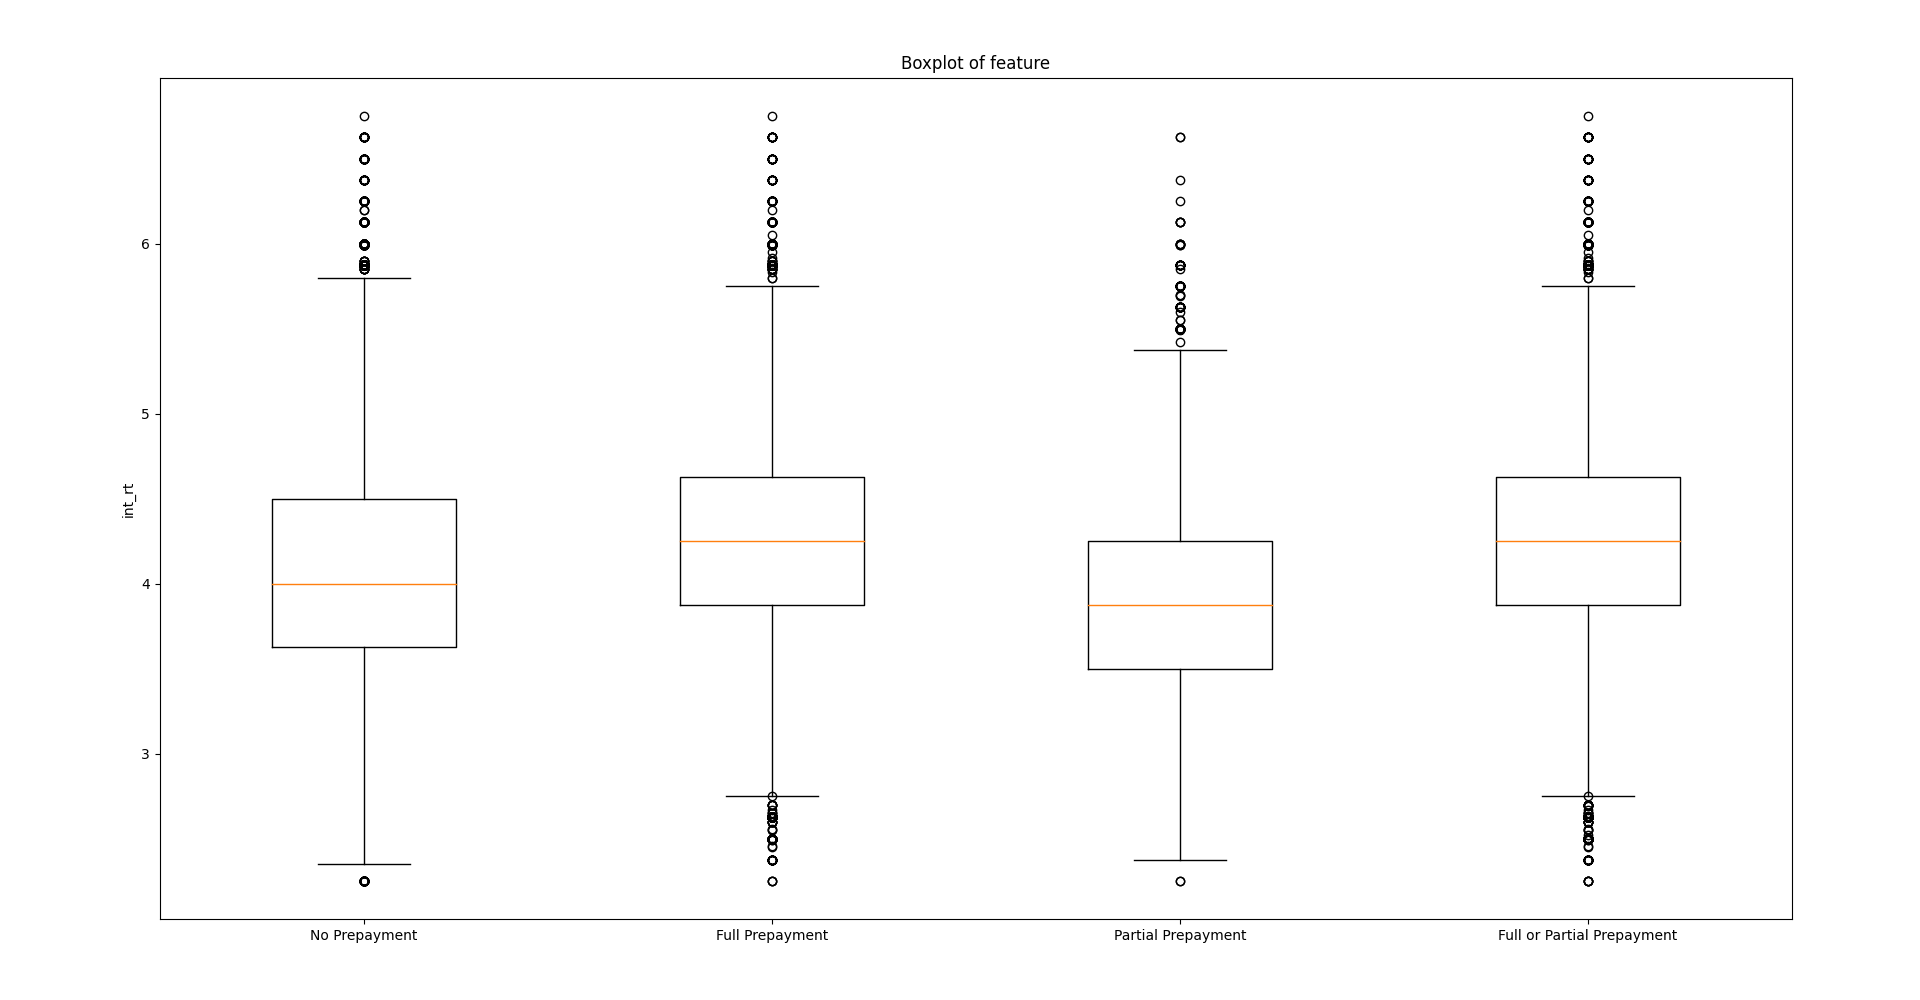
\includegraphics[width=\linewidth]{Latex/Report/Figures/Boxplot_of_int_rt_[2013, 2014, 2015, 2016, 2017, 2018, 2019, 2020]_.png}
            \caption{Boxplot of original interest rate of sample data. From left to right: No prepayment, Full prepayment, Partial prepayment and Full or Partial prepayment.}
            \label{model_boxplot_int_rt}
        \end{figure}
        \noindent
        The influence of the original interest rate of year 2013 can be seen in Figure \ref{model_int_rt_against_prepayment}. Here, one observes again a higher interest rate implying more prepayments. Note the interest rate for full prepayments to be higher than the interest rate of partial prepayments. 
        \begin{figure}[H]
            \centering
            \begin{subfigure}{0.45\textwidth}
                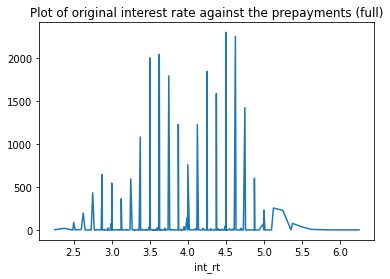
\includegraphics[width=\linewidth]{Latex/Report/Figures/int_rt againts Full prepayments.png}
                \caption{Interest rate against Full prepayments.}
                \label{model_int_rt_against_full_prepayment}
            \end{subfigure}
            \begin{subfigure}{0.45\textwidth}
                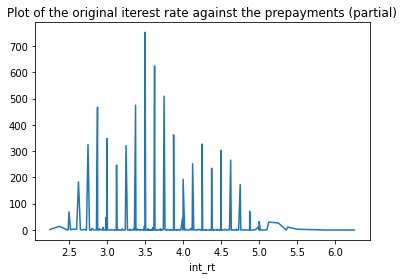
\includegraphics[width=\linewidth]{Latex/Report/Figures/int_rt againts Partial prepayments.png}
                \caption{Interest rate against Partial prepayments.}
                \label{model_int_rt_against_partial_prepayment}
            \end{subfigure}
            \caption{Original interest rate against magnitude of prepayments.}
            \label{model_int_rt_against_prepayment}
        \end{figure}
        
    
    

    




    \newpage
    
    \section{Model}\label{section_model}
    Using the analysis of the data set discussed in the previous 
section, the model can be constructed. First, a discussion is given 
about the requirements for the models. After this, the theoretical 
framework around the model is given. In this framework the logistic 
regression is considered. In the theoretical framework, also the 
methodology with respect to addressing the performance is described.
The logistic regression model is suggested by the company. 
For this reason this model is chosen as main model to test with respect 
to the data.  

\subsection{Model Description} \label{subsec_model_descr}
    % Modelling the prepayment probabilities. 
    The model will predict prepayment probabilities. 
    Generally, results of the model will be obtained in the following 
    way. 
    First, there is a variable selection. Based on this variable
    selection, certain features will be used in predicting the prepayment  
    probabilities. The selected features will be on a client level and 
    can be used to estimate the specific probabilities of prepayment 
    on a client level. Both the full and the partial prepayment will 
    be estimated, i.e. the probability that a client with certain 
    characteristics will do a partial or full prepayment. 
    As the data also includes time dependence, a set up which also 
    takes time into consideration will be discussed. To this extend, 
    suppose a portfolio $P$ with client data, a time step $t$ on 
    which the estimation will be performed and a future time horizon $T$. 
    Using the data up to the moment $t$, for the whole portfolio, 
    the model will perform an estimation of the probabilities per 
    client over the given time horizon $T$. 
    \\\\ 
    % Getting the input data
    As described in Section \ref{section_data_analysis}, 
    the total data set can be split in two data sets. One for the 
    client data given at $t_0$ (which is referred at as
    the originate data set) and one which contains information of 
    the mortgage over time (which is referred to as the monthly 
    data set). For a client $i$ in $P$ the data provides certain 
    information at moment that the mortgage is closed. These variables
    will be denoted as  $x_1^i, \ldots, x_n^i$ 
    Also there is time dependent information, these variables will be 
    denoted as  $x_1^{t, i}, \ldots, x_m^{t, i}$. As for all the clients, 
    the same procedure 
    is used, the $i$ is omitted for convenience, hence 
    $x_k^i \equiv x_k$ and $x_l^{t, i} \equiv x_l^t$ for each 
    $k \in \{1, \ldots, n\}$ and $l \in \{1, 
    \ldots m \}$.  The fixed time information can be inferred
    from the originate data and the time dependent data can be 
    inferred from the monthly data. As the model evaluate the data on 
    a specific time step, it can evaluate the features 
    $x_1, \ldots, x_n$ directly. On the other hand, the data
    which depends on time cannot be used directly and needs to be 
    transformed. This transformation will be such that each feature 
    on a certain time step includes all the information up to that 
    moment. To get this information, a certain condition $c_k$ is set. 
    For all time steps $t_i < t$, this condition will be verified 
    over the data. To bring it to one number on time $t$, the 
    evaluations of the condition over all time steps will be aggregated 
    using some aggregation operator. To make this more clear, consider 
    the following example. Suppose a client $i \in P$ and the feature 
    $x^{t_i}$, which describes if the prepayment type (i.e. no, partial or 
    full) at time $t_i$. Now, consider the condition $c_k$:
    \begin{equation}
        c_k(x^{t_i}) = \left\{
        \begin{array}{l l l l l}
            1 & \text{if there is a partial prepayment at time } t_i \\ 
            0 & \text{else}
        \end{array}
        \right.
    \end{equation}
    Evaluating this condition, over all time steps $t_i$ up to the moment 
    $t$ and summing over those evaluations, yield a new feature $x$. 
    This feature represents the count of partial prepayments up to time 
    $t$ for that client. Now $x$ can be used as a feature to predict 
    the prepayment probabilities for this client. 
    \\\\
    % Addressing the output
    As described above, the model returns prepayment probabilities 
    (partial, full and no prepayment)for a specific client. More 
    specifically, suppose a random variable $Y$ which can take values in 
    $\{0, 1, 2\}$ where $Y=0$ is no prepayment, 
    $Y=1$ is a partial prepayment and $Y=2$ represents a full prepayment. 
    The model will return the probabilities 
    $P(Y = 0 | X) = p_0, P(Y = 1 | X) = p_1$ and 
    $P(Y = 2 | X) = p_2$
    for given features $X = [x_1, \ldots, x_{n+e}]$ (where the number of 
    features 
    $n+e$ is based on the derived features from the monthly data and 
    the variable selection). The predicted probability 
    $p_j, \ j \in \{0, 1, 2\}$ is the probability 
    that that prepayment state will be hit by the client within the 
    interval $[t, T]$. 

\subsection{Multinomial logistic model}
    For the purposes of this assignment, we used the multinomial logit model; 
    a generalisation of the binomial logistic regression for a target 
    variable of more than two classes. In our case, the classes we have are three: No Prepayment, Partial Prepayment and Full Prepayment. We considered a nominal model instead of an ordinal one because, despite the fact that a Full Prepayment is a prepayment of higher magnitude than a Partial Prepayment, they are events that differ in nature. 
    
    We assume that our categories are encoded as 0 for No prepayment, 1 for Partial Prepayment and 2 for Full Prepayment. 0 is going to be our reference class. Therefore, our model will yield to logit functions, one for each of the other two classes and the probability of class 0 will be calculated by subtracting the sum of the two probabilities from 1.
    
    The two logit functions, $g_1, g_2$ will then be:
    \begin{equation}
        g_1(x) = ln\Big[\frac{Pr(Y=1|x)}{Pr(Y=0|x)}\Big] = \beta_{10} + \beta_{11}x_1 + \beta_{12}x_2 +...+ \beta_{1p}x_p = x^T\beta_1
    \end{equation}
    
    \begin{equation}
        g_2(x) = ln\Big[\frac{Pr(Y=2|x)}{Pr(Y=0|x)}\Big] = \beta_{20} + \beta_{21}x_1 + \beta_{22}x_2 +...+ \beta_{2p}x_p = x^T\beta_2
    \end{equation}
    
    If we then consider $g_0 = 0$ the conditional probabilities for each class j, $j=0,1,2$ will be given by:
    
    \begin{equation}
        p_j(x) = Pr(Y=j|x) = \frac{e^{g_j(x)}}{\sum_{j=0}^{2} e^{g_j(x)}}
    \end{equation}
    
    The coefficients vector are then computed after deriving the maximum likelihood. The likelihood is constructed as follows. $Y=0$ when $Y_0=1$, $Y_1=Y_2=0$, $Y=1$ when $Y_1=1$, $Y_0=Y_2=0$ and $Y=2$ when $Y_2=1$ and $Y_0=Y_1=0$. Then, the conditional likelihood is derived by:
    \begin{equation}
        l(\beta) = \prod_{i=1}^{n}[p_0(x_i)^{y_{0i}}p_1(x_i)^{y_{1i}}p_2(x_i)^{y_{2i}}] 
    \end{equation}
    
    Then the log-likelihood is:
    \begin{equation}
        L(\beta) = \sum_{j=1}^{n} y_{1i}g_1(x_i) + y_{2i}g_2(x_i) - ln(1 + e^{g_1(x)} + e^{g_2(x)})
    \end{equation}
    
    By taking partial derivatives one can then compute the maximum likelihood and therefore the $\beta$ coefficients. \cite{logistic}
    
    
    % \textcolor{red}{(Theory part)}

    Initially, we aggregated all our originate data, that is the data 
    sets that contain information for specific loans as mentioned in 
    Section \ref{section_data_analysis}.

    We then split the data set into two separate ones. A train set 
    which contained 70\% of the observations of the data set and which 
    we used to train our model and a test set, containing the rest of 
    the observations and which we used to assess the performance of the 
    model.
    From those, we will train our model in the 
    Because of the nature of our variables, even after the random split of our dataset, we keep only those 

    % \textcolor{red}{\subsection{Possible second model if time allows}}


\subsection{Variable selection}
    For reasons of computational time, to avoid possible overfitting 
    and to have an alternative model to compare with our initial one, 
    we thought of selecting a subset of feature. We used the LASSO 
    multinomial regression. Lasso stands for least absolute shrinkage 
    and selection operator. Multinomial LASSO, just as LASSO regression 
    tends to shrink not important variables and keep only those that 
    are significant in the final model. 
    %For a system of equations 
    %\begin{equation}
     %   Y=X\beta +\epsilon  
    %\end{equation}
    %the lasso estimator is defined by
    %\begin{equation}
     %   \min_\beta(||Y-X\beta||^2+\lambda||\beta||_1).  
    %\end{equation} 
    %$\lambda$ denotes the penalty given by lasso regression and 
    %determines the bias of the estimator. 
    In the multinomial case we consider an extension of the method. 
    In this case, there are more than one levels need to consider. 
    While working with $K$ levels, in the multinomial case, one uses 
    the following probability function:
    \begin{equation}
        Pr(G=k|X=x)=\frac{e^{\beta_{0k}+\beta_k^T x}} {\sum_{l=1}^K e^{\beta_{0l}+\beta_l^T x}}  
    \end{equation}
    By setting $p_l(x_i)=Pr(G=l|x_i)$, $g_i\in \{1,2, \hdots, K\}$ and to
    maximize the log-likelihood after taking partial derivatives, one needs to maximize \parencite{Friedman_2010}: 
    \begin{equation}
        \max_{\{\beta_{0k},\beta_k\}_1^K}
        \left[
            \frac{1}{N}\sum_{i=1}^N 
            \log(p_{g_i}(x_i))-\lambda \sum_{l=1}^K P_\alpha (\beta_l) 
        \right].  
    \end{equation}
    This function can be rewritten as
    \begin{equation}
        l(\{\beta_{0k},\beta_k\}_1^K)=
        -\left[ 
            \frac{1}{N} \sum_{i=1}^N
            \left( 
                \sum_{k=1}^Ky_{il}(\beta_{0k}+x_i^T\beta_k)-
                \log\left(
                    \sum_{l=1}^K e^{\beta_{0l}+x_i^T\beta_l}
                \right)
            \right)
        \right],  
    \end{equation} 
    in which $Y$ is the $N\times K$ indicator response matrix. 
    Matrix $Y$ consists of $y_{ik}=I(g_i=l)$ \parencite{Friedman_2010}. 
    \\\\
    In this case, the penalized negative log-likelihood 
    function for the LASSO case in the elastic net context is given by 
    \parencite{hastie2016introduction}:
    \begin{equation}
        l(\{\beta_{0k},\beta_k\}_1^K)=
        -\left[ 
            \frac{1}{N} \sum_{i=1}^N\left( 
                \sum_{k=1}^Ky_{il}(\beta_{0k}+x_i^T\beta_k)-
                log\left(
                    \sum_{l=1}^K e^{\beta_{0l}+x_i^T\beta_l}
                \right)
            \right)
        \right] + \lambda \sum_{j=1}^p ||\beta_j||_q.  
    \end{equation}

    % \textcolor{red}{Variable selection obtained with lasso}

\subsection{Performance criteria}
    % \textcolor{red}{ROC-AUC}
    To assess the performance of our model we used an extension of 
    the ROC curve for multiple classes. In the typical binomial ROC 
    plot, we can calculate the AUC, that is the Area Under the (ROC) 
    Curve, as follows. Consider $p(x)$ the probability that x belongs 
    to class 0. If $f(p)=f(p(x)|0)$ the probability function of 0 
    class points belonging to class 0 and $g(p(x)|1)$ the probability 
    function of class 1 points belonging to class 0, then we can plot 
    their corresponding cumulative distributions F and G against each 
    other.
    
    The resulting plot with $G(p)$ on the vertical axis and $F(p)$ on 
    the horizontal is the ROC curve. If the ROC curve lies above the 
    positive slope diagonal, then we have a better than random model. 
    The area under the curve is then our AUC. A perfect model would 
    yield an AUC of 1, a random one 0.5 and a completely wrong one 0.
    For multiclass prediction models, plotting the ROC curve is not 
    really feasible. But since the AUC can be computed directly from the  is obtaining the AUC is possible, extending the 
    definition to more classes. Considering $i=0,1,2,...,c-1$ classes 
    with $c>2$, and $p(i|x)$ the respective probability functions. 
    For any pair of classes $i$ and $j$, we define $A(i|j)$ as the 
    probability that a randomly selected observation from the jth class 
    will have a lower estimated probability of belonging to class $i$ 
    than a randomly drawn member of class $i$.\cite{handtill2010}
    \\\\
    For the two class case, obviously $A(i|j) = A(j|i)$. But it 
    doesn't generally hold.
    \begin{equation}
        A(i|j)=\frac{S_i-n_i(n_i+1)/2}{n_in_j},  
    \end{equation}
    where $n_i$ is the number of observations within the ith class.
    \begin{equation}
        A(i,j) = \frac{1}{2}(A(i|j)+A(j|i)).   
    \end{equation}
    Then, the overall AUC is given by the M measure, where 
    \begin{equation}
        M=\frac{2}{c(c-1)}\Sigma_{i,j}A(i,j)
    \end{equation}
    
    % \textcolor{red}{AIC}
    
    Akaike's Information Criterion, aka AIC, is obtained by the 
    following equation:
    \begin{equation}
        AIC = 2k-2ln(L)  
    \end{equation}
    where k is the number of predictors and L is the maximum value 
    of the likelihood function for the model. Goodness of fit is 
    assessed by the likelihood function and then penalized by the 
    number of parameters to avoid overfitting. Thus, between two models 
    having a similar maximum likelihood, the one with fewer parameters 
    will be preferred based on the AIC measure.
    \newpage
    
    \section{Results}\label{section_results}
    For the purposes of this report we have built two models. One, is the model utilising every variable we have had available, either from the original datasets provided, or the new ones we have created as mentioned in Section. The second one, utilises those that have remained non zero after applying LASSO regression. This way, we can make a comparison between the two.

The variables that had non zero coefficients with lambda.1se in the LASSO regression are 57. They include: cntUnits, cltv, dti, ltv, ppmtPnlty, cntBorr, flagSc, flagFTHBY, occpyStsP, channelR, several states, servicer and seller names and type of property. In total, they are 57, reducing the number from the initial 197 to almost a quarter. 


    \csvautolongtable[
        table head=\caption{some table}\label{tab:some}\\\hline
        \csvlinetotablerow\\\hline
        \endfirsthead\hline
        \csvlinetotablerow\\\hline
        \endhead\hline
        \endfoot,
        respect all
    ]{CSV/FullCOefficients.csv}
    
In Table \ref{ModelAICandAUC}, we can see that the reduced model, not only performs worse in terms of AUC, but in addition, its AIC increases, despite the reduction of parameters. This means that our reduced model's likelihood has decreased and the fit of the reduced model is no better than the complete one.
    
    \begin{table}[H]
        \centering
            \begin{tabular}{c|c|c}
            Model & AUC & AIC \\\hline
            Complete Model & 0.8253303 & 70606\\
            LASSO Reduced Model &  0.7838138 & 72473\\
            
		    \end{tabular}
            \caption{AUC and AIC values for different input parameters.}
	        \label{ModelAICandAUC}
    \end{table}

    \newpage
    
    \section{Discussion}\label{section_discussion}
    \subsection{Recommendation for further research}
    As in this project only one model is used, there is no 
    extensive research done on other models that could be 
    used for classification. For instance, a random forest 
    model or a neural network could also be possible models 
    to address the prepayment probabilities. These models 
    could be further researched to possibly obtain more accurate 
    results. 
    \\\\
    Besides different models which do simple classification, 
    also time dependent models could be considered (e.g.
    auto regressive models), to use this kind of models 
    however, more time based data about the client is 
    needed. One can think of personal information like age
    and income, but also information about the property over 
    time. As this is information that cannot be provided in 
    an open source data set, we were not able to work with 
    this information. However, a bank can have access to 
    this kind of information and may be able to optimize
    the models using this data.
    For data that is less accessible, the bank can also 
    make use of simulation to obtain estimates of client 
    specific information. One can think of estimating the 
    fico on a client level using copulas which depend
    on client information.
    \\\\
    Furthermore, as noted before, the modelling is done 
    with a selected sample of the available open-source 
    data set provided by FreddieMac. An analysis between 
    the sample set and the full data set should be done 
    to determine if the sample is representable for the 
    whole set. 
    \\\\ 
    As the LASSO seems not to give that good results for 
    selecting risk drivers, other methods of variable 
    selecting could be considered. Due to time constraint 
    it was not possible to include this into this report. 
    However, one could try to use other models which 
    address variable importance to do variable selection. 
    For example, a random forest could be used for this. 
    \newpage
    
    \printbibliography
    \newpage
    
    % Appendices
    \appendix
    \input{Appendices/ExampleAppendix.tex}

\end{document}
